\section{Monte Carlo Simulation}
It has been already mentioned, that MC approaches can be used to research many body systems which are not solvable analytically.
Numerical methods simplify this task, but they introduce other challenges - in most cases (especially for large scaling sizes), it is not possible to acces every single state.
However, for the explanation of the used algorithm, this can be neglected for now.

\subsection{Detailed Balance and the Metropolis Algorithm}
Consider the particle flow out of state $\ket{i}$
\begin{align}
	j^\text{out}_{i} \mathrel{\mathop:}= \sum_j P_i(t) W_{ij},
\end{align}
with jump probability $W_{ij}$ from state $\ket{i}$ to $\ket{j}$.
Analogue, the particle flow into state $\ket{i}$ can be written as
\begin{align}
	j^\text{in}_{i} \mathrel{\mathop:}= \sum_j P_j(t) W_{ji}.
\end{align}
This yields to the master equation
\begin{align}
	\frac{\mathrm{d}P_i(t)}{\mathrm{d}t} = 
		\sum_{j}\left(P_j(t)W_{ji} - P_i(t)W_{ij}\right),
\end{align}
which is fulfilled in the equilibrium (left hand side vanishs) by the stricter condition of detailed balance\footnote{This is a strong, but not necessary condition to prevent the resulting Markov chain to be trapped in a limit cycle~\cite{newman1999monte}.}
\begin{align}
	P_iW_{ij} = P_jW_{ji}.
\end{align}
In other words - the system moves towards equilibrium if detailed balance is enforced\footnote{But not in the classical, newtonian way of motion, every snapshot of the system towards equilibrium is the result of random initialised trial steps.}.
The key of success is to choose $W_{ij}$ such that detailed balance is fulfilled.
This is accomplished with the Metropolis Criterion
\begin{align}
	W_{ij} = \left\{
		\begin{array}{c l}
			\exp(-\beta\Delta E)&\text{, if}\Delta E = E_j - E_i > 0\\
			1										&\text{, if }\Delta E \leq 0 
		\end{array}\right..
\end{align}
The according proof is short accepting $\Delta E > 0$ without qualification
\begin{align} 
	\frac{W_{ij}}{W_{ji}} = \frac{\exp\left(-\beta\Delta E\right)}{1} = \frac{\exp(-\beta E_j)}{Z}\cdot\frac{Z}{\exp(-\beta E_i)} = \frac{P_j}{P_i}.
\end{align}

\subsubsection*{Explanatory Note}
This criterion does always accept the trial state, if the energy is lowered and exponentially suppresses those, which raise the energy.
For the sake of illustration, all simulation steps will be described in detail.
\begin{enumerate}
	\item{Initialise the coordinates of all particles - random or sorted}
	\item{Perform $M$ trial moves $(M \approx\,??)$, i.e.
		\begin{itemize}
			\item{Select a particle and move it with vector $\delta r$}
			\item{Compute the energy difference $\Delta E = E_j - E_i$}
		\end{itemize}
	\item{Generate a uniformly distributet random number $x$ in $[0, 1]$ and accept the trial move, if eighter $\Delta E>0$ or $x < \exp(-\beta\Delta E)$, discard otherwise.}
}
\end{enumerate}

\begin{figure}[ht]
	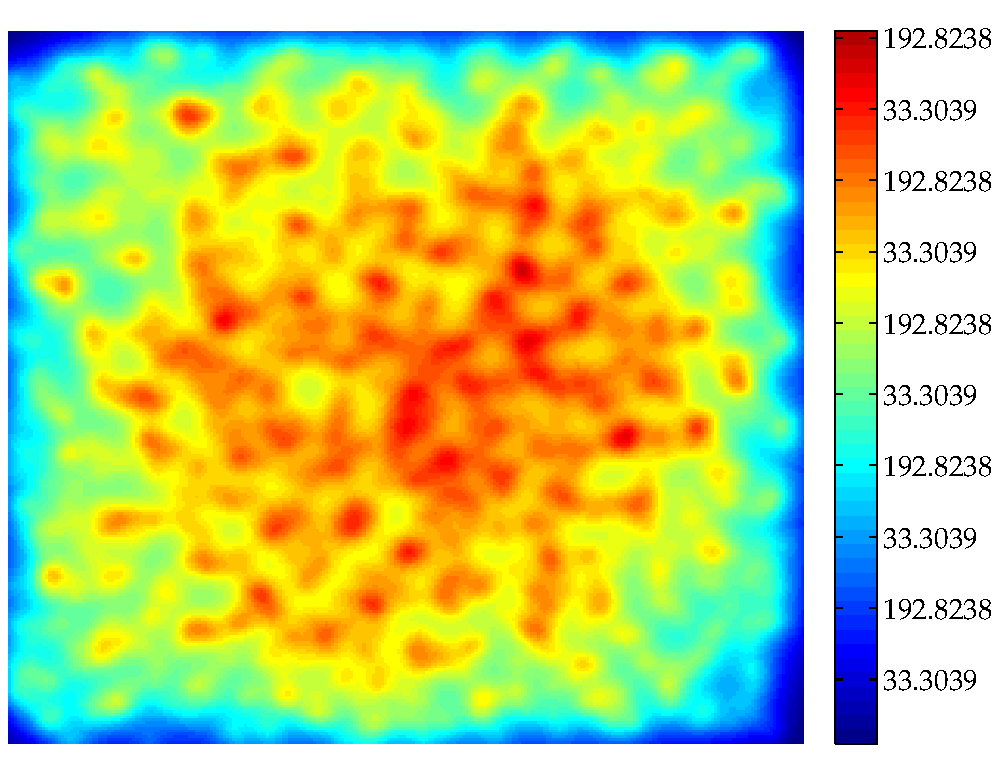
\includegraphics[width=\textwidth]{Figures/TestFrame.pdf}
\end{figure}
% \subsection{Convergency Behaviour}
